\begin{evenBlock}{1v1 Evade with Help}

\begin{minipage}[t]{\linewidth}
    \centering
    
    \begin{minipage}{.5\linewidth} % Left column and width
        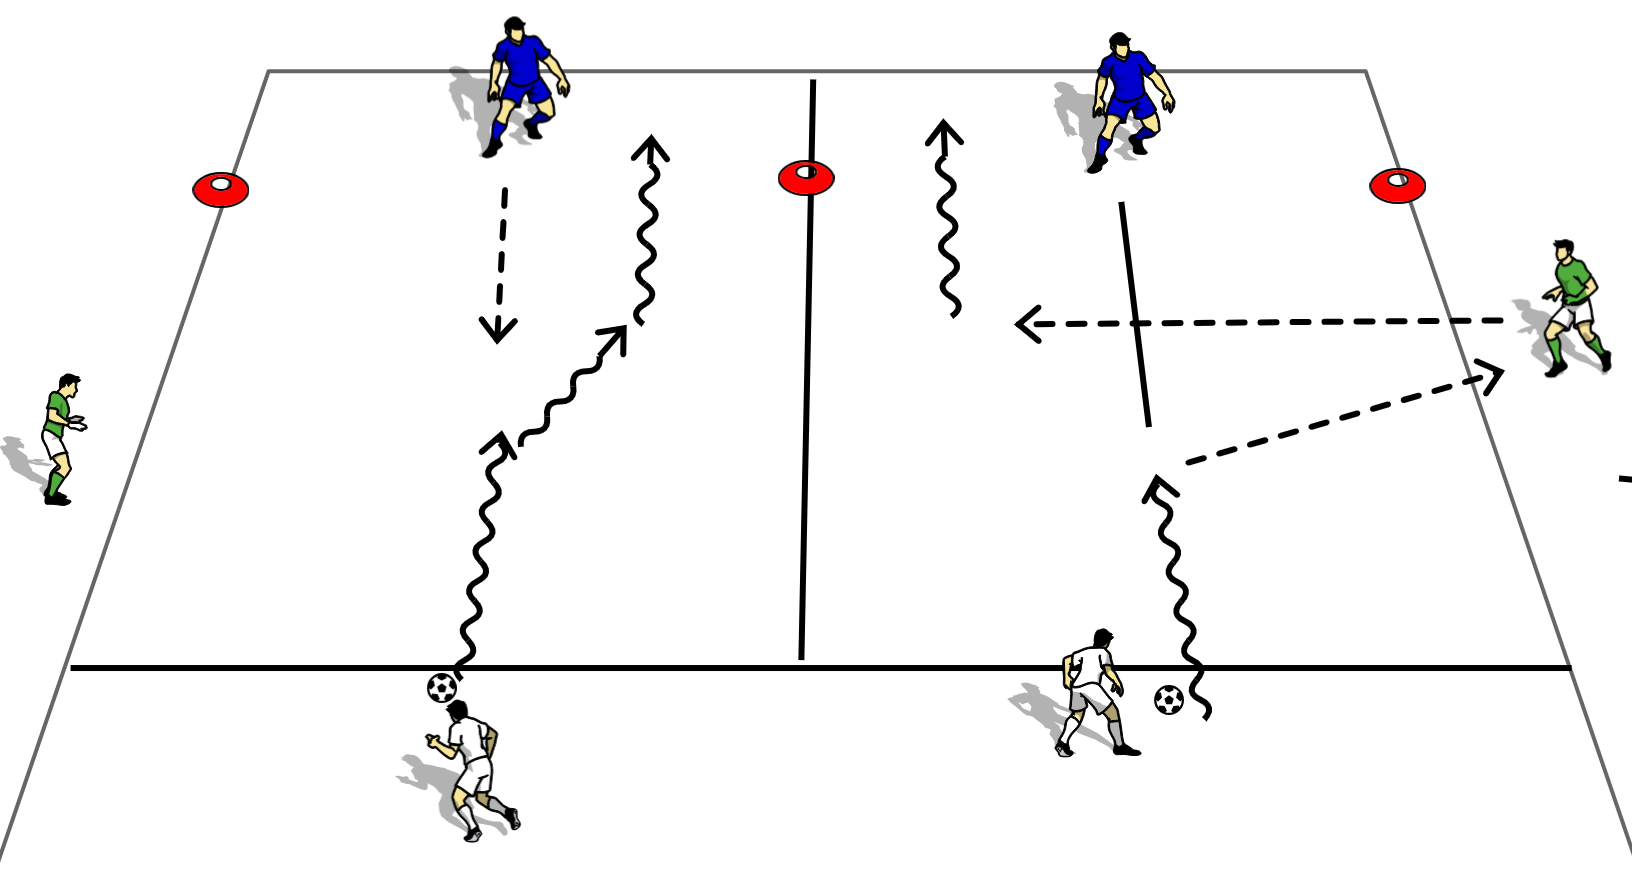
\includegraphics[width=\textwidth]{../img/Trimmed/Evade_1V1+Help}
    \end{minipage}
    \hspace{0.05\linewidth}
    \begin{minipage}{.4\linewidth} % Left column and width
        \textbf{Drill Description:}
        The object is to get the ball (the snitch) and take it across the opposite end line.
        \begin{enumerate}
            \setlength{\itemsep}{0pt}
            \setlength{\parskip}{0pt}
            \setlength{\parsep}{0pt}
            \item Player with the ball crosses the far end line and ties to dribble across the opposite endline.
            \item A defender starts behind the red cones and can cross them as soon as the attacker enters the box.
            \item The attacker needs to evade the defender or pass to his helper (coach) on the side line, who one touches the ball back into play.
        \end{enumerate}
    \end{minipage}
\end{minipage}
\vspace{12pt}

\textbf{Coaching Points:}
\begin{itemize}
    \setlength{\itemsep}{0pt}
    \setlength{\parskip}{0pt}
    \setlength{\parsep}{0pt}
    \item The timing of the attacking move is critical, it needs to be early enough to insure the defender can't block it, but not so early the defender can react to counter it.
    \item Use the pass as a great opportunity to evade the defender.
\end{itemize}
\end{evenBlock}